\documentclass[a4paper,10pt,twocolumn,upLatex]{jsarticle}
\usepackage{style/campus_presen_resume}
\usepackage{multirow}
\usepackage{hhline}
\usepackage{comment} 
\usepackage{scalefnt}
\usepackage{cite}

\newenvironment{minilinespace}{
\baselineskip = 4mm
}

%---------------------------------------------------------------------
%編集者用(変更不要)
%1:修士論文諮問会 2:卒業論文発表会counter
\type{2}
\year{2021}
\month{2}
\date{20}		%day{}にする
%---------------------------------------------------------------------
\setcounter{page}{1}
%---------------------------------------------------------------------

\begin{document}
%---------------------------------------------------------------------
%各自タイトル作成部分(要変更)
%\makesubtitle{タイトル}{title}{名前}{name}{name}
\makesubtitle{3次元環境認識に基づく死角領域内のAR可視化によるドローン操縦性向上}
{Improving Drone Maneuverability by AR Visualization in Blind Spot Areas Based on 3D Environmental Awareness}{竹内一真}{Kazuma} {Takeuchi}

%---------------------------------------------------------------------
%---------------------------------------------------------------------

\section{はじめに}
近年,多方面でのドローンを活用した事業が進出しており,中でも小型ドローンは小さな機体を活かして,人が入れない狭小空間での活躍の場も増えることが考えられる.しかし,狭小空間でのドローンの飛行は遮蔽物が多く,遮られた視点からの操縦を必要とし操縦は困難な場合がある.
オンボードカメラ搭載のドローンを使用する場合では,安全な距離から狭小空間を探索することができるが,ドローン視点の操縦では前方以外の死角が多くなり,状況認識が不十分である\cite{FPV}欠点がある.
そこでAR(Augmented Reality)を用いて死角領域を可視化することで,操縦者視点での操縦を行える.しかし,操縦者視点での操縦を実現する上で,障害物までの距離感を掴めない懸念がある.
\par
そこで本研究では,操縦者の死角領域内を可視化し,ドローン近傍の障害物を検知するAR方式を提案することで,操縦者がどのような情報によって,安全にドローンを操縦できるかを検討する.

%---------------------------------------------------------------------
\section{関連研究}
\subsection{Drone-Augmented Human Vision}
Eratらの研究では,狭小空間でのビデオストリーミング映像を基にしたドローン視点の一人称での操縦が困難ということで,HoloLensを通して壁を透過した,操縦者視点の三人称でのドローン操縦を提案している\cite{AR_drone}.
結果として,一人称視点での条件と比較して三人称視点での条件の方が課されたタスクの完了までの操縦時間が半分以下となることが分かった.

\subsection{問題点}
障害物を考慮しない環境を想定してあり,障害物などによる危険性が提示されていない.また,2つの条件間での操縦法が異なるため,操縦時間への有意差がARによる空間認識によるものかどうかが不確かである.よって衝突の危険性を提示し,ドローン操縦法を統一することで,ARによってドローン操縦性向上を示せるかどうかを検討する必要がある.

%---------------------------------------------------------------------
\begin{figure}[t]
\begin{center}
  \scalebox{0.43}{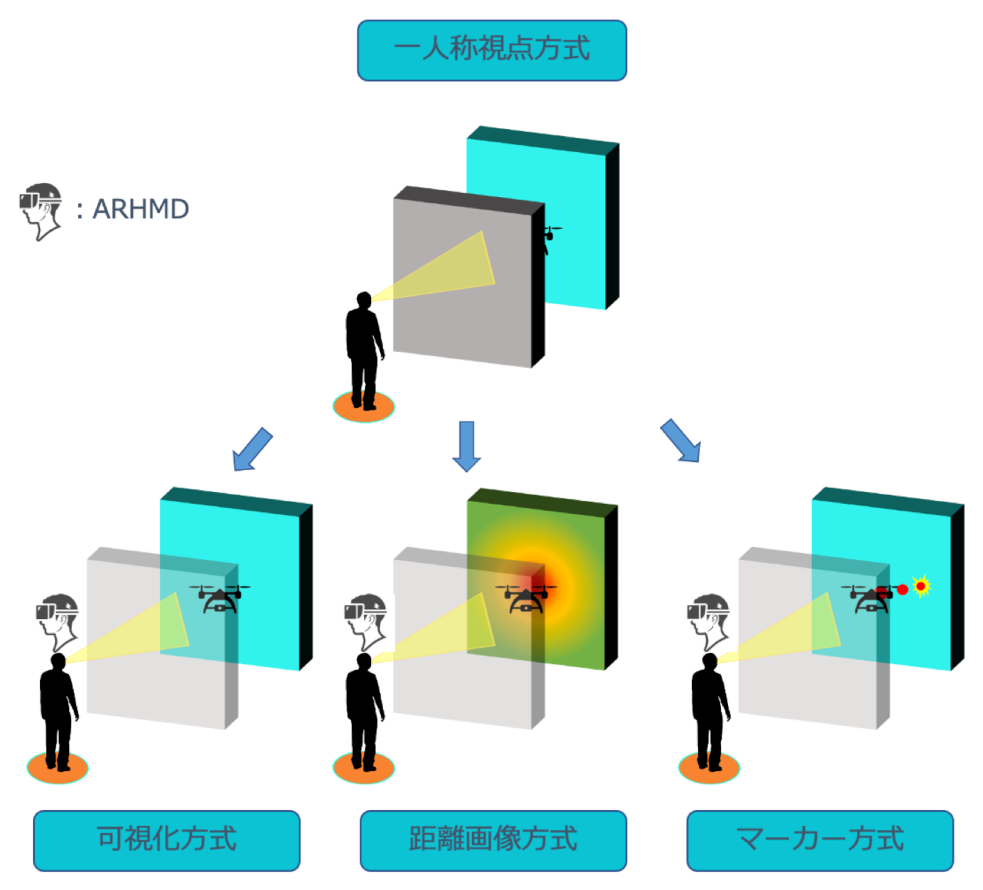
\includegraphics{img/Overview.eps}}\vspace{-2mm}
  \caption{各方式の動作例}
  \label{fig:flow}
\end{center}
\end{figure}
%---------------------------------------------------------------------

\section{死角領域内でのドローン操縦}
\subsection{一人称視点方式}
一人称視点方式では,従来のドローン操縦に用いる操縦法を使用する.操縦者はドローンから配信されるビデオストリーミング映像を基に,ドローン中心の一人称視点での操縦を行う.

\subsection{可視化方式}
可視化方式では,3次元環境を事前に入手し,ARによって3次元環境とドローンを重畳表示し,遮蔽物を透過することで,操縦者への死角領域の空間認識を提供する.

\subsection{距離画像方式}
距離画像方式は,可視化方式に加えて近傍の障害物を知覚するために,人間の奥行き知覚を支援する.ステレオビジョンを参考にしており,ドローンから障害物までの距離に応じて,障害物の色を分けている.

\subsection{マーカー方式}
マーカー方式は,可視化方式に加えて近傍の障害物を知覚するために,どの方向の障害物が危険かの直感的な理解を支援する.ドローンから見て最も近い障害物に対して,目印を付けている.


\begin{figure}[tb]
\begin{center}
  \scalebox{0.4}{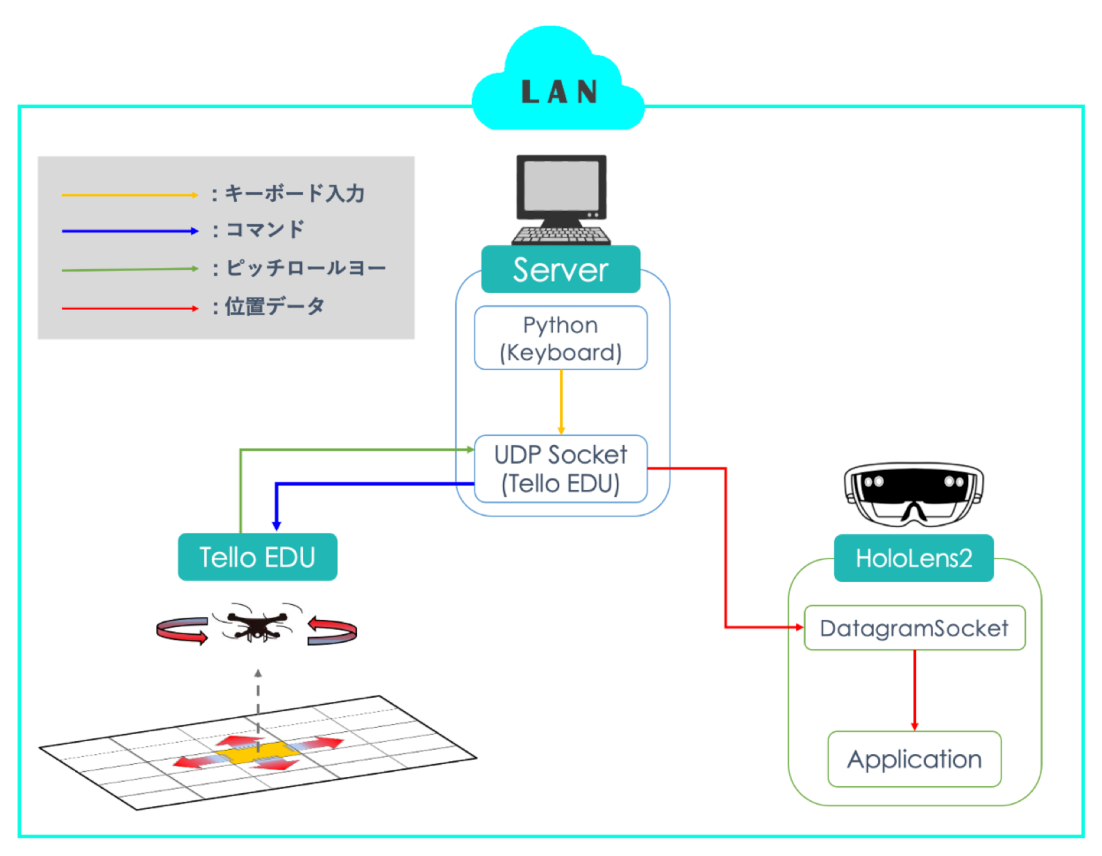
\includegraphics{img/flow.eps}}\vspace{-2mm}
  \caption{システム構成}
  \label{fig:overview}
\end{center}
\end{figure}

%---------------------------------------------------------------------
%---------------------------------------------------------------------
\section{評価}\label{experiment}
\subsection{実装}
提案手法のシステム構成を図\ref{fig:overview}に示す.
ドローンはTello EDU,
ARHMDはMicrosoft HoloLens2,
サーバはMacBookProを使用する.
事前にHoloLens2のSpatial Mappingにより空間マッピングを行い,静的な3次元環境地図を作成する.
サーバでは常時Tello EDUの傾きや,移動距離をHoloLens2に送信することで,3D仮想空間上に存在するドローンの位置合わせを行っている.
\par
距離画像方式,マーカー方式では共に障害物までの距離によって,危険度を色で示している.操縦者がドローンを操縦する際の衝突する危険性がある距離が0.3mと示されている\cite{obstruct}ため,距離画像方式では,障害物までの距離が0.3mまでを赤色,0.3m\textasciitilde0.6mまでを黄色,0.6m以上を緑色で示す.マーカー方式では障害物までの距離が0.3mまでを赤色のマーカー,0.3m\textasciitilde 0.6mの際に黄色のマーカーを示す.

%---------------------------------------------------------------------
%---------------------------------------------------------------------

\subsection{実験}
実験参加者はドローンをスタート地点から操縦し,目的地点で着陸するタスクを行った.その間,衝突の恐れのある障害物を設置し,衝突することなく正確に通過することを要求した.
各方式での,タスクを完了するまでの操縦時間,障害物への衝突警告回数,参加者へのアンケートを記録した.操縦時間には一次元配置分散分析(ANOVA)を用いてデータを分析した.また,ポストホック検定では,TukeyのHSD検定を行い,各方式の比較を行なった.衝突警告回数では,Friedman 検定を行い,Bonferroni法の多重比較検定を行い各方式の比較を行なった.

%---------------------------------------------------------------------
%---------------------------------------------------------------------

\subsection{評価と考察}
操縦時間の結果を図\ref{fig:time},衝突警告回数を図\ref{fig:collision}に示す.ARを利用した方式ではARなしの方式と比較して一貫して平均の操縦時間が有意に減少し,可視化方式を除いて衝突警告回数が有意に減少したことがわかった.このことより,ARを用いた方式は死角領域内でのドローン操縦に置いて有効である.また,AR方式同士の比較では,距離画像方式が最も操縦時間が短く衝突警告回数が少ないことが分かる.本研究で使用するようなドローンは最大飛行時間が短く,その間に操縦をすることを求められる中で,距離画像方式は,従来の操縦法である一人称視点方式と比較して操縦時間が約30\%減少したことより,大幅に作業効率を向上させることが見込まれる.また距離画像方式は,ドローン操縦において衝突を無くす必要がある中で衝突警告回数を0であったことから,実際の死角領域内の狭小空間においても有効であることを示した.

%---------------------------------------------------------------------
%---------------------------------------------------------------------
\begin{figure}[tb]
\begin{center}
  \scalebox{0.58}{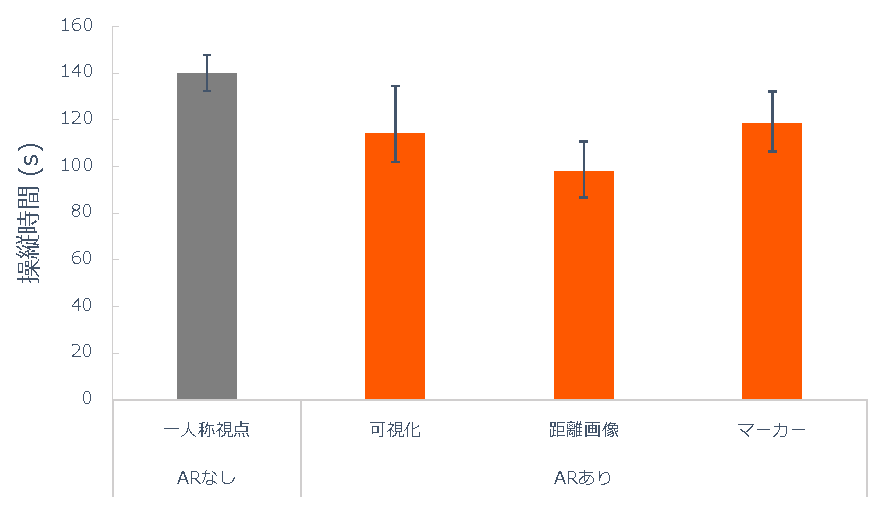
\includegraphics{img/time.eps}}\vspace{-2mm}
  \caption{タスク完了までの操縦時間}
  \label{fig:time}
\end{center}
\end{figure}

\begin{figure}[tb]
\begin{center}
  \scalebox{0.54}{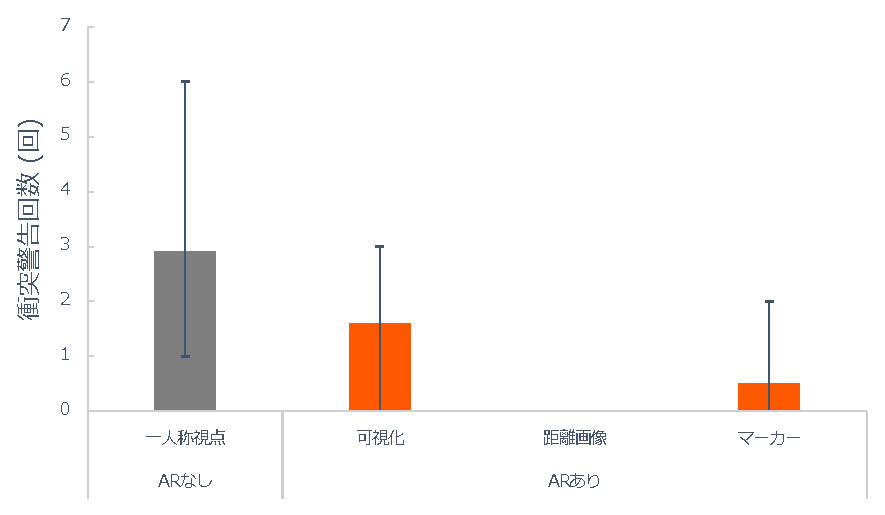
\includegraphics{img/collision.eps}}\vspace{-2mm}
  \caption{衝突警告回数}
  \label{fig:collision}
\end{center}
\end{figure}
%---------------------------------------------------------------------
%---------------------------------------------------------------------
\section{まとめ}
小型ドローンでの遮られた視点からの狭小空間での操縦は死角の多さや,ドローンと障害物までの距離感が測れないことが懸念されている.本研究では操縦者の死角領域内に存在するドローンと周辺を可視化し,ドローン周辺の障害物を知覚するためのAR方式を提案し,実験を行うことで,遮られた視点からの狭小空間でのドローン操縦性を評価した.結果として,ARを利用した方式では操縦時間が短く,衝突回数も少なかったことから操縦性の向上が確認された.
また,障害物を知覚するためのAR方式では,ドローン周辺の障害物に危険度を振り分けている方式が操縦者へ安心感を与え,操縦性の向上を示した.
%---------------------------------------------------------------------
%---------------------------------------------------------------------

{\footnotesize 
\begin{thebibliography}{99}
\bibitem{FPV}
S. A. Green, J. G. Chase, X. Chen and M. Billinghurst, "Evaluating the Augmented Reality Human-Robot Collaboration System", 2008 15th International Conference on Mechatronics and Machine Vision in Practice, Auckland, pp. 521-526, 2008

\bibitem{AR_drone}
O. Erat, W. A. Isop, D. Kalkofen and D. Schmalstieg, Drone-Augmented Human Vision: Exocentric Control for Drones Exploring Hidden Areas, in IEEE Transactions on Visualization and Computer Graphics, vol.24, no.4, pp.1437-1446, 2018.

\bibitem{obstruct}
山田開斗, 薄羽大樹, 宮下芳明, "ドローン操縦におけるクロッシング評価", 研究報告ヒューマンコンピュータインタラクション(HCI), Issue.2, No.2, pp.1-6, 2019

\end{thebibliography}
}
\end{document}
%---------------------------------------------------------------------
